\documentclass{article}
\usepackage[utf8]{inputenc}
\usepackage{amsmath}
\usepackage{amsfonts}
\usepackage{graphicx}
\usepackage{listings}

\title{%
    1º Projeto da disciplina Estruturas de Dados II \\
     \large Análise assintótica de algoritmos de ordenação}
\author{Gabriel Passarelli 11218480\\ Marcelo Kenji Noda Pique Pique, tchururu}
\date{2021}

\begin{document}
%
\maketitle
%
\newpage
\section{Introdução}
Nosso objetivo com este texto é analisar a complexidade de tempo de cinco algoritmos de ordenação distintos, implementados na parte prática do projeto em linguagem C de programação seguindo os pseudo-códigos fornecidos na proposta do trabalho.\par
%
Em cada seção, fazemos a análise de maneira teórica do pseudo-código de um algoritmo, dando ênfase para o comportamento assintótico da complexidade de tempo, e em seguida apresentamos os resultados obtidos a partir das medições de tempo feitas rodando os códigos implementados. Nessa parte, incluímos gráficos e tabelas para facilitar a visualização dos dados.
%
\section{Análise dos algoritmos}
\subsection{Bubble Sort (versão otimizada)}
O procedimento de ordenação do Bubblesort tem por base comparar elementos adjacentes, e invertê-los, caso o último seja menor do que o primeiro. Paramos de percorrer o vetor comparando as posições contíguas se não houverem mais trocas a serem realizadas (e isso distingue o Bubblesort otimizado do normal). Fato é que a cada laço em que se torna a percorrer o vetor, não caminhamos até seu fim, mas sim até uma posição antes à que foi atingida no laço anterior. De fato, não é necessário ir até o fim, já que após $i$ rodadas os $i$ maiores elementos estarão ocupando as posições corretas no vetor.\par
%
De modo mais preciso, vemos no pseudo-código da rotina Optimized\_Bubble\_Sort que, no pior caso, dado um vetor de tamano $n \in \mathbb{N}$ o número de operações será $n$ vezes o custo do for da linha $4$. Este, por sua vez, realizará aproximadamente 
\[\sum_{i = 0}^{i = n-1}6\cdot(n-i-2) = 3(n - 3)n\] operações em seu interior (a operação de troca normalmente se utiliza de uma variável auxiliar, de modo que o custo dela se torna o custo de 3 atribuições). Ou seja, temos um custo total, no pior caso, $O(n^2)$.\par
O pior caso caso acontece somente quando o vetor está ordenado de maneira decrescente. Tomando um vetor aleatório podemos obter o caso médio. Nessa situação, a probabilidade de que uma elemento esteja ocupando uma dada posição no vetor no começo é $1/n$. Além disso, se ele está deslocado $j$ posições de sua posição correta, então precisaremos realizar pelo menos $j$ trocas para acertá-la. A questão que precisamos responder então é: em média, quantas posições um elemento está deslocado de sua posição correta? Seja $X_k$, a variável aleatória que mede a distância de um elementos a sua posição correta, quando está é $k$. Temos \[E[X_k] = \sum_{i = 0}^{k-1}\frac{(k-i)}{n}+\sum_{i = k+1}^{n}\frac{(i - k)}{n} = \frac{n+k^{2}+(n-k)^{2}}{2n},\] logo, em um vetor de tamanho $n$, realizaremos \[\sum_{i=0}^{n}E[X_k] = \sum_{i=0}^{n}\frac{n+k^{2}+(n-k)^{2}}{2n} = \frac{(n+1)(n+2)}{3×} = O(n^2)\] permutações.\par
%
Nossas medições de tempo confirmam nossas análises téoricas, como bem se vê pela inclinação das retas do gráfico que segue
%
\begin{figure}[h]
    \centering
    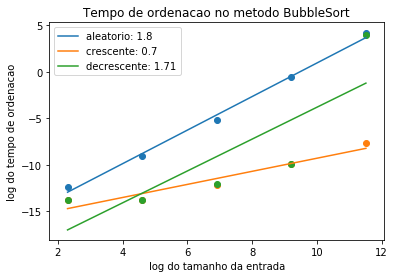
\includegraphics[width=0.6\textwidth]{bubble_sort.png}
    \caption{Os números na frente das legendas indicam as inclinações das respectivas retas. Como esperado, os gráficos para entradas aleatórias e ordenadas de modo decrescente aprenentam comportamento próximo ao quadrático, enquanto entradas já ordenadas têm comportamento próximo ao linear.}
\end{figure}
%
\begin{table}[h]
    \begin{tabular}{c|c|c|c|c|c}
        n = & $10^{1}$ & $10^{2}$ & $10^{3}$ & $10^{4}$ & $10^{5}$ \\ 
        \hline
        Vetor aleatório & $4\cdot 10^{-6}$ & $1.15\cdot 10^{-4}$ & $5.28\cdot 10^{-3}$ & $5.47\cdot 10^{-1}$ & $61.04$ \\
        \hline
        Vetor crescente & $10^{-6}$ & $10^{-6}$ & $5\cdot 10^{-6}$ & $5.1\cdot 10^{-5}$ & $4.61\cdot 10^{-4}$\\
        \hline
        Vetor decrescente & $10^{-6}$ & $10^{-6}$ & $6\cdot 10^{-6}$ & $5\cdot 10^{-5}$ & $52.17$\\
        \hline
        Média & $2\cdot 10^{-6}$ & $3.9\cdot 10^{-5}$ & $1.76\cdot 10^{-3}$ & $1.82\cdot 10^{-1}$ & $37.7$ \\
        \hline
        Desvio Padrão & $1.41\cdot 10^{-6}$ & $5.37\cdot 10^{-5}$ & $2.49\cdot 10^{-3}$ & $2.58\cdot 10^{-1}$ & $26.92$ \\
    \end{tabular}
    \caption{Medidas de tempo para o Bubblesort em segundos}
\end{table}\par
Observando a tabela, podemos notar como o desvio padrão cresceu junto com o aumento do tamanho da entrada. Isso reforça nossa avaliação de que a complexidade do BubbleSort está altamente relacionada ao número de elementos ocupando suas posições corretas previamente.
\subsection{Quick Sort}
Pique Pique, tchururu
\subsection{Radix Sort}
A ideia básica por trás do Radixsort é ordenar nossos inteiros de modo recursivo, usando como chave de ordenação uma casa decimal diferente a cada chamada. Além disso, comeaçamos pelo dígito menos significativo e terminamos no dígito mais significativo. Cabe dizer também que é claro que nossas entradas não precisam ser inteiros: datas também funcionariam, por exemplo, ou qualquer outro dado que pudesse ser interpretado como uma sequência de caracteres com uma relação de ordem entre si.\par
%
No pseudo-código, começamos com um vetor $A$ de tamanho $n$. A codição $(maior/posicao)>0$ é, pelo que dissemos acima, a condição de parada do processo de ordenação: $A$ está ordenado quando $posicao$ tiver mais dígitos do que o maior elementos de $A$. Usamos a rotina Counting\_Sort como auxiliar. Ela é responsável por ordenar o vetor $A$ considerando apenas a casa decimal das entradas do vetor dada pela fórmula $\log_{10} posicao$. Note que, portanto, o $enquanto$ da linha 4 do peseudo-código rodará um número de vezes igual ao número de dígitos do maior elemento contido em $A$.\par
%
A rotina Counting\_Sort tem como lógica inferir a posição correta de um dado elemento $a$ de $A$ através da contagem de quantos elementos menores do que $a$ existem em $A$, e é exatamente essa a informação que $B$ guarda: na primeira iteração, contamos quantos elementos de $A$ possuem o dígito especificado pela variável $posicao$ igual a $i$; no segundo laço de iterações contamos também quantos elementos com o dito dígito menor do que $i$ existem em $A$, e salvamos essa informação em $B[i]$. Assim, é evidente que o número correto da posição de $A[i]$ será exatamente $B[chave] - 1$, em que $chave$ é o dígito considerado na chamada atual. Note que a cada iteração, decrementa-se o valor guardado em $B[chave]$, de modo a não se perder os elementos de $A$ com dígito atual igual. No algoritmo, o vetor $C$ serve apenas como auxiliar ao processo de inverção das posições do elemento de $A$.\par
%
\begin{figure}[h]
    \centering
    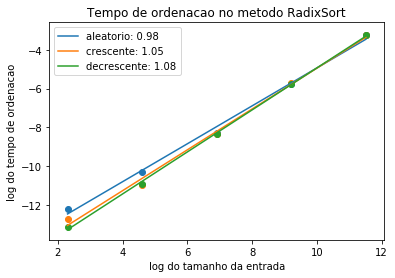
\includegraphics[width=0.6\textwidth]{radix_sort.png}
    \caption{Como esperado, a inclinação de todas as retas é próxima de 1, indicando o comportamento linear.}
\end{figure}
%
É fácil ver que a complexidade do Radix\_Sort não se altera de acordo com o número de elementos já ordenados no vetor: não fazemos comparações dos elementos entre si, mas sim um procedimento de contagem, cuja complexidade depende apenas do tamanho de $A$. Assim, a complexidade total do algoritmo será, para qualquer vetor de tamanho $n$ \[s\cdot\left[(8 \cdot n + 1) + (1 + 9\cdot4) + (1 + 9\cdot n) + (1 + 3\cdot n)\right] = O(n),\]
em que $s$ corresponde ao número de dígitos do maior elemento do vetor.
%
\begin{table}
    \begin{tabular}{c|c|c|c|c|c}
        n = & $10^{1}$ & $10^{2}$ & $10^{3}$ & $10^{4}$ & $10^{5}$ \\ 
        \hline
        Vetor aleatório & $5\cdot 10^{-6}$ & $3.4\cdot 10^{-5}$ & $2.53\cdot 10^{-4}$ & $3.15\cdot 10^{-3}$ & $3.96\cdot 10^{-2}$ \\
        \hline
        Vetor crescente & $1.7\cdot10^{-5}$ & $10^{-6}$ & $2.42\cdot 10^{-4}$ & $3.3\cdot 10^{-3}$ & $3.89\cdot 10^{-2}$\\
        \hline
        Vetor decrescente & $1.8\cdot10^{-5}$ & $10^{-6}$ & $2.43\cdot 10^{-4}$ & $3.12\cdot 10^{-3}$ & $3.89\cdot 10^{-2}$\\
        \hline
        Média & $3.33\cdot 10^{-6}$ & $2.3\cdot 10^{-5}$ & $2.46\cdot10^{-4}$ & $3.2\cdot 10^{-3}$ & $3.92\cdot 10^{-2}$ \\
        \hline
        Desvio Padrão & $1.24\cdot 10^{-6}$ & $7.78\cdot 10^{-5}$ & $4.97\cdot 10^{-6}$ & $7.89\cdot 10^{-5}$ & $3.31\cdot 10^{-4}$ \\
    \end{tabular}
    \caption{Medidas de tempo para o RadixSort em segundos}
\end{table}\par
%
Na tabela, ressaltamos os valores pequenos para o desvio padrão, que indicam que as medidas não se alteraram muito quando mudamos a forma de preencher o vetor a ser ordenado. Isso reforça a ideia de que a complexidade é a mesma para dois vetores quaisquer de mesmo tamanho.
\subsection{Heap Sort}
Pique Pique, tchururu
\end{document}
